\subsection{Miluphcuda SPH code}
Miluphcuda is a smoothed particle hydrodynamics code that has been developed over several years at the University of Tuebingen by Christoph Schaefer and others. Its general use is well documented in \cite{Schaefer_2016}.


\subsection{Initial conditions}
- Target basalt halfsphere
- Impactor aluminium sphere
- resolution bound to variable smoothing length
- Uniform macro structure but random micro structure to avoid
- seagen \cite{github:SEAGen} used to create initial conditions

\begin{figure}[H]
    \centering
    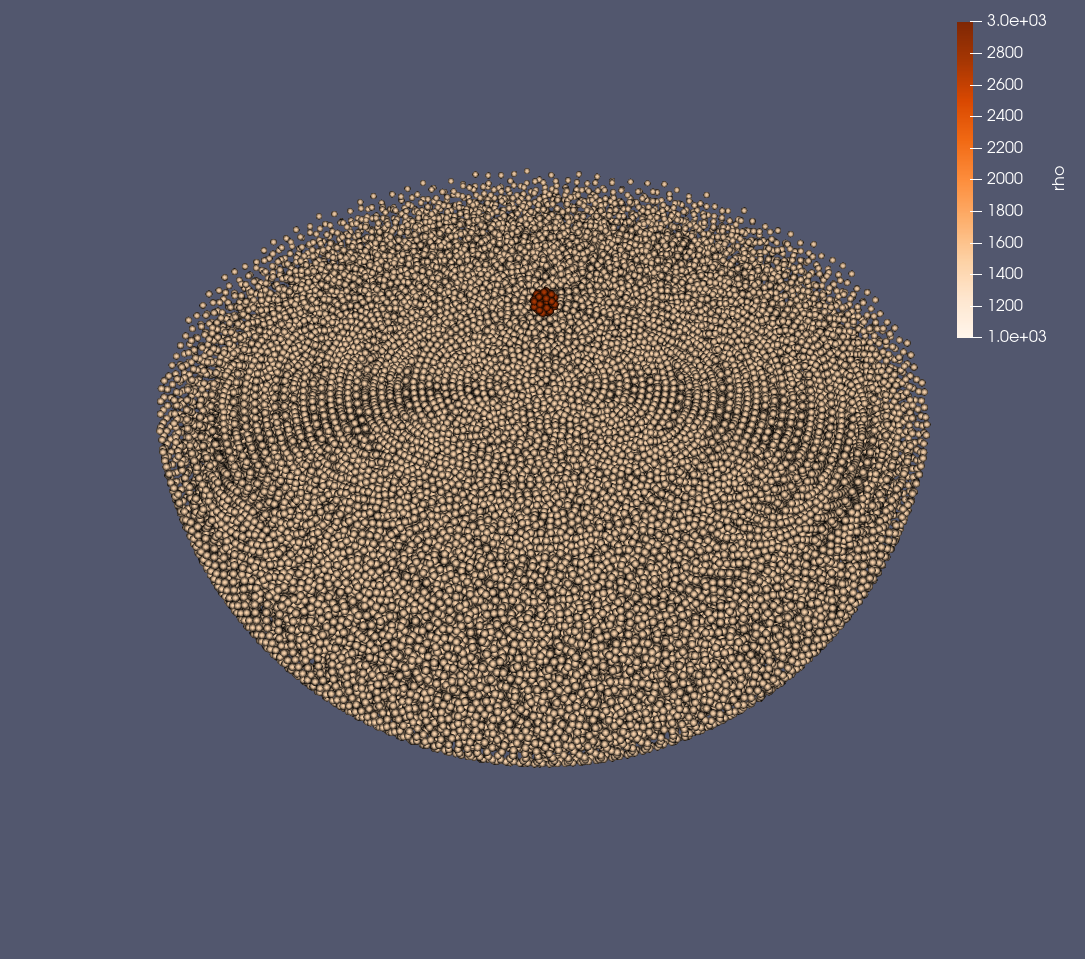
\includegraphics[width=\textwidth]{impact_start.png}
    \caption{start of simulation}
    \label{fig:impact_start}
\end{figure}

\begin{figure}[H]
    \centering
    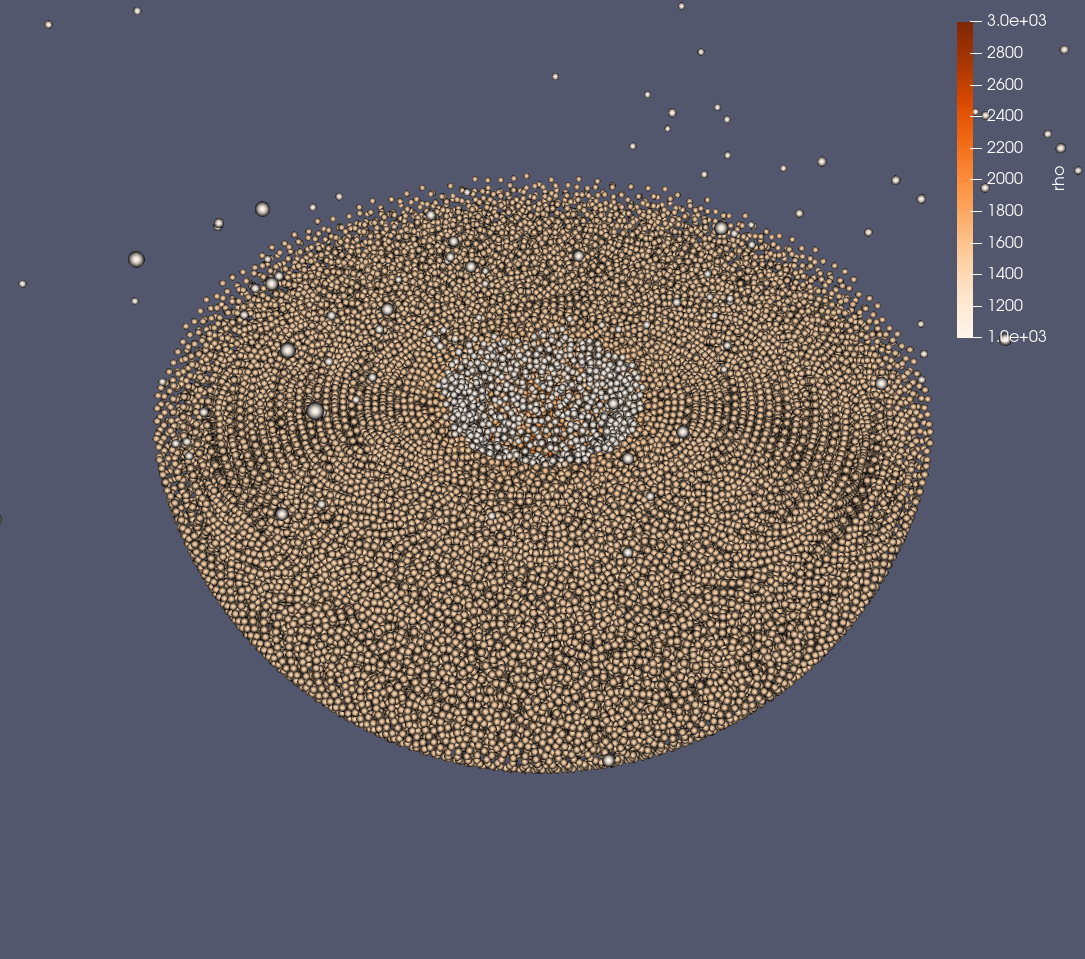
\includegraphics[width=\textwidth]{impact_end.png}
    \caption{end of simulation}
    \label{fig:impact_end}
\end{figure}

\subsection{Material parameters}

\begin{table}
    \centering
    \begin{tabular}{ |l|l|l|l| }
        \hline
        \multicolumn{2}{|c|}{}                & Target                  & Projectile                                                          \\
        \hline
        \multirow{10}{*}{Tillotson EOS}       & $\rho_0$                & 2.86 $\cdot 10^3 g\cdot cm^{-3}$ & 2.70 $\cdot 10^3 g\cdot cm^{-3}$ \\
                                              & $A_T$                   & 2.67 $\cdot 10^{10}$ Pa          & 7.52 $\cdot 10^{10}$ Pa          \\
                                              & $B_T$                   & 2.67 $\cdot 10^{10}$ Pa          & 6.50 $\cdot 10^{10}$ Pa          \\
                                              & $E_0$                   & 4.87 $\cdot 10^8$ J              & 5.00 $\cdot 10^6$ J              \\
                                              & $E_{iv}$                & 4.72 $\cdot 10^6$ J              & 3.00 $\cdot 10^6$ J              \\
                                              & $E_{cv}$                & 1.82 $\cdot 10^7$ J              & 1.39 $\cdot 10^7$ J              \\
                                              & $a_T$                   & 0.5                              & 0.5                              \\
                                              & $b_T$                   & 1.5                              & 1.63                             \\
                                              & $\alpha_T$              & 5.0                              & 5.0                              \\
                                              & $\beta_T$               & 5.0                              & 5.0                              \\ \hline
        \multirow{7}{*}{Porosity}             & $\alpha_0$              & \textbf{varying}                 & not porous                       \\
                                              & $p_{elastic}$           & 1.0 $\cdot 10^6$ Pa              & not porous                       \\
                                              & $p_{transition}$        & 6.8 $\cdot 10^7$ Pa              & not porous                       \\
                                              & $p_{compacted}$         & 2.13 $\cdot 10^8$ Pa             & not porous                       \\
                                              & $\alpha_e$              & 4.64                             & not porous                       \\
                                              & $\alpha_t$              & 1.90                             & not porous                       \\
                                              & $c_s$                   & 100.0 $m\cdot s^{-1}$            & not porous                       \\ \hline
        \multirow{6}{*}{Strength}             & cohesive strength $Y_c$ & \textbf{varying}                 & 1.0 $\cdot 10^9$ Pa              \\
                                              & $\alpha$                & 0.982793 rad                     & 0 rad                            \\
                                              & $\alpha_{damaged}$      & 0.540419 rad                     & 0 rad                            \\
                                              & shear modulus $\mu$     & 2.27 $\cdot 10^{10}$ Pa          & 2.69 $\cdot 10^{10}$ Pa          \\
                                              & bulk modulus $K_0$      & 2.67 $\cdot 10^{10}$ Pa          & 5.23 $\cdot 10^{10}$ Pa          \\
                                              & yield stress $Y_0$      & 3.5 $\cdot 10^9$ Pa              & 2.76 $\cdot 10^8$ Pa             \\ \hline
        \multirow{2}{*}{Weibull}              & M                       & 16                               & no damage                        \\
                                              & K                       & 1.0 $\cdot 10^{61}$              & no damage                        \\ \hline
        \multirow{2}{*}{Artificial viscosity} & $\alpha$                & 1.0                              & 1.0                              \\
                                              & $\beta$                 & 2.0                              & 2.0                              \\ \hline
        \hline
    \end{tabular}
    \caption{Material parameters for basalt target and aluminium Impactor}
    \label{fig:material_parameters}
\end{table}

- variable smoothing length min 0.1 bis max 10.0
- rholimit 0.95